\documentclass{article}
\usepackage{fancyhdr,booktabs}
\usepackage{amsmath}
\usepackage{float}
\usepackage{graphicx}
\usepackage{indentfirst}
\usepackage{geometry}
\usepackage{citesort}


\begin{document}
\title{Can We Build the Light Sail for the Travel to Proxima b?}
\author{Team 335}
\date{\today}
\maketitle

\begin{abstract}
	A potentially habitable planet, Proxima b, was found in 2016 and sending spacecraft for scientific research for this planet has been discussed in the past two years. Using ground-based laser beam array to power a light sail into space is one promising project. In this paper, we discussed the relativistic dynamics during the acceleration stage and performed several numerical simulations. We choose several parameters to characterize accuracy, precision and uniformity of laser array, as well as engineering details of the light sail. In order to hit the planet within earth-moon distance from Solar-Proxima distance (4.365 light year), the constraints on the parameters are unbelievably strict. In conclusion, it's extremely hard to build the proper light sail and establish the laser array within required accuracy.
\end{abstract}


\section{Introduction}

Proxima b, a planet discovered in 2016, orbits the nearest star from our sun, Proxima, every 11 days. After the discovery, several projects for performing scientific research on the planet are proposed. However, due to long interstellar distance, even though Proxima is the nearest star from us, it would take up to 100 years to reach the planet with traditional spacecraft.  

Solar sail, a type of space craft using light pressure provided by luminous objects, such as a star and optical devices. Recently a new conception of interstellar solar sail has been proposed, i.e. using laser array on the ground to accelerate a micro space craft which is a few gram of mass. Such a space craft could reach high velocity in a few minutes and an interstellar voyage might be realized.

The stability of the dynamics in acceleration stage is considered in \cite{stab}. Their conclusion is conic shaped sail is stable in the acceleration dynamics. Therefore we also use conic sail in our simulation. The deceleration of the craft at Proxima system is considered in \cite{dec}. The light pressure of the stars in Alpha Centauri system can be used to decelerate the craft so that the payload can even land on the planet other than flyby at high speed.

There's still some problems unsolved because of long distance from . First, the accuracy and precision of the laser beam should be high so that the light spot can aim at the sail from ground. Second, the precision should be even higher to reach exactly the desired velocity, otherwise the craft might miss the Proxima b. Theoretically the laser beam is Gaussian, the optimized standard division $\sigma$ should be considered. An additional problem is the uniformity of laser beam, a small deviation of angles between different beams in the array could cause similar problems.

We consider both Newtonian and relativistic condition, maximize the standard devision of Gaussian beam. We also care about the accuracy and the maximum error of laser beam array's direction are given. We consider the uniformity as a random Gaussian perturbation in laser's unit direction vector and the minimum uniformity are founded.

\section{Analysis and Simulation}
\subsection{non-relativistic system}

A sketch graph is shown at Fig.1,as discussed in \cite{},the non-relativistic equations of motion are:
\begin{align}
\boldsymbol{F} &= \int_S 2\frac{P( \boldsymbol{x'})\hat{\boldsymbol{b}}\cdot\hat{\boldsymbol{n}}(\boldsymbol{x'})}{c}\cdot\hat{\boldsymbol{n}}dS \\
\boldsymbol{F} &= m\boldsymbol{\ddot{x}}
\end{align}
where $\boldsymbol{F}$ is total force of sail, $m$ is mass of sail, $S$ is surface of sail, $P$ is power flux of laser beam, $\boldsymbol{x'}$ is position of laser reflection point, $\boldsymbol{x}$ is position of mass center of sail, $\hat{\boldsymbol{b}}$ is unit vector along the beam, $\hat{\boldsymbol{n}}$ is unit vector perpendicular to the reflection surface\\
\begin{figure}[htpb]
	\centering
	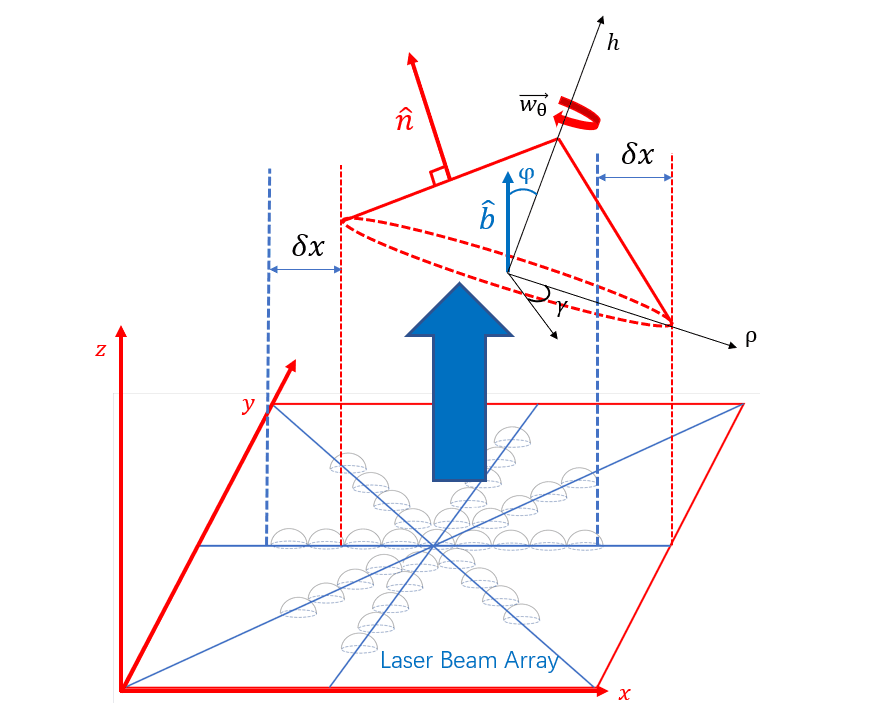
\includegraphics[scale=0.3]{scheme.png}
	\caption{sketch graph of sail,coordinate $Oxyz$ is static with laser beam and $O'\rho\gamma h$ is along with sail}
\end{figure}
in the coordinate $O'\rho\gamma h$,the value of $\hat{\boldsymbol{n}}$ is:
\begin{equation}
\hat{\boldsymbol{n}} = 
\begin{pmatrix}
&cos\alpha sin\phi +sin\alpha cos\gamma cos\phi\\
&sin\alpha sin\gamma\\
&cos\alpha cos\gamma - sin\alpha cos\gamma sin\phi
\end{pmatrix}
\end{equation}
By some geometric tricks, the reflection point is(along with $Oxyz$):
\begin{equation}
\boldsymbol{x} = \boldsymbol{x'} + 
\begin{pmatrix}
&\rho sin\alpha\\
&\rho cos\gamma\cos\phi -(\frac{H}{2}-\rho tan\alpha)sin\phi\\
&\rho cos\alpha sin\phi + (\frac{H}{2}-\rho tan\alpha)\cos\phi
\end{pmatrix}
\end{equation}
where:$\alpha$ is inclination angle of sail and $H$ is height of sail\\


\subsection{relativistic system}
Taking relativity into consideration, given the momentum $\vec{k}$, the forces are given by (see Appendix for the derivation) :
\begin{equation}
	F_{//}=\int_S \frac{P(x) +P_f \cos (2\beta) }{c} dS 
\end{equation}
\begin{equation}
	F_{\perp}=\int_S \frac{P_f \sin (2\beta)}{c} dS \\
\end{equation}
$F_{//}$ is the component parallel to the momentum and $F_\perp$ is the component perpendicular to the momentum.
$P_f$ is given by:
\begin{equation}
	P_f=\frac{P(x) \sqrt{m^2c^4+|\vec{k}|^2c^2 } - P(x)|\vec{k}|c \cos(\alpha- \beta) }{P(x)dt (1-\cos(1\beta)) +\sqrt{m^2c^4+|\vec{k}|^2c^2 } + |\vec{k}|c \cos(\alpha- \beta) }
\end{equation}

where $\alpha$ is the angle between $\vec{k}$ and $\hat{n}$, $\beta$ is the angle between $\hat{b}$ and $\hat{n}$ and $P(\vec x)$ is the power flux at location $\vec x$

Then with the relativistic definition of momentum:
\begin{equation}
	\vec k = \frac{m \vec v}{\sqrt{1-v^2/c^2}}
\end{equation}
\begin{equation}
	\vec{F} = \frac{d \vec k}{dt}
\end{equation}
we have the relativistic equation of motion. 

\subsection{simulation result}
We use relativistic equations to perform numerical simulations, namely integrating the first order ODE (reduced from second order by doubling variants) with RK4(5) method. The result is shown in Fig \ref{sim1}. From the data, the craft could reach desired velocity in 819.1 seconds. Parameters of this system are set as listed in Table. \ref{par1}, some of the parameters are defined in Chapter 3.

\begin{table}[!htb]
	\centering
	\label{par1}
	\caption{Parameters set in Simulation 1}
	\begin{tabular}{lllllll}
		\toprule
		m	&S	&$\alpha$	&$x_0$	&$y_0$	&$\sigma_P$	&$\sigma_b$\\
		\midrule
		10g	&10$m^2$	&0	&0	&0	&1.25m	&0\\
		\bottomrule
		
	\end{tabular}
\end{table}

\begin{figure}[]
	\centering
	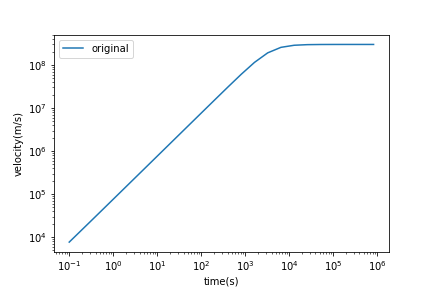
\includegraphics[width=12cm]{simu.png}
	
	\caption{velocity evolution. The velocity reaches 60860120.67 m/s at 819.1 seconds}
	\label{sim1}
\end{figure}


\section{Marginal Error}
	In order for the craft to hit Proxima b within earth-moon distance, the deviation of velocity should satisfy following criteria:
	\begin{itemize}
		\item Direction: the direction should be within angle that 2 earth-moon distance has at 4.365 light year (distance from earth to Proxima). 
		\item Amplitude: the time required to reach Proxima b at the speed should not lag or lead the desired value to much so that the craft misses the planet due to revolution around Promixa. 
	\end{itemize}
	Therefore, we have :
	\begin{equation}
		\Delta \theta \le \frac{2*d_{earth-moon}}{4.365 l.y.}
	\end{equation}
	\begin{equation}
		\frac{4.365l.y.}{v_0}- \frac{4.365l.y.}{v_0+\Delta v}\le \frac{2d_{earth-moon}}{2\pi a} T
	\end{equation}
	where $d_{earth-moon}$ is the distance between earth and the moon, $v_0$ is 0.2 light speed as desired, a is the semi latus rectum of the Proxima b's orbit and T is the period of the orbit.
	
	So the marginal error in the velocity is:
	\begin{equation}
		\Delta \theta \le 1.862 \times 10^{-8} rad
		\,\,\,\,\,\,\,
		\Delta v \le 4.58 \times 10^{-7} c
	\end{equation}
	where c is light speed.
	
	In order to satisfy this strict constraint, the system should be carefully calibrated. Here we list the parameters we choose to quantify the system:
	\begin{itemize}
		\item Accuracy of beam array: central position of power flux distribution $(x, y)$
		\item Precision of beam array: Gaussian variance of the power flux distribution $\sigma$
		\item Fabrication of the light sail: The area $S$ and the conic angle $\alpha$
		\item Uniformity of the laser beam: the Gaussian variance of $\vec{b}$, $\sigma_b$
	\end{itemize}
	
	In the simulation discussed in last section, we perturb the parameters listed above by a small amount and observe the resulted velocity, which are then used to calculated partial derivatives. The velocity evolution of several perturbed cases are shown in Figure. \ref{pert}. The results of derivations and marginal errors are listed in Table. \ref{pd}
	
	\begin{figure}[]
		\centering
		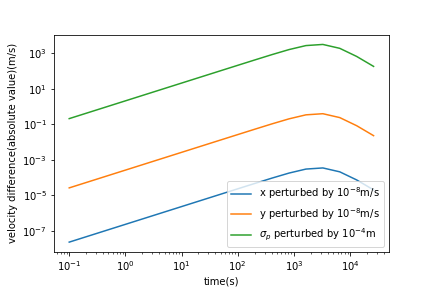
\includegraphics[width=12cm]{pert.png}
		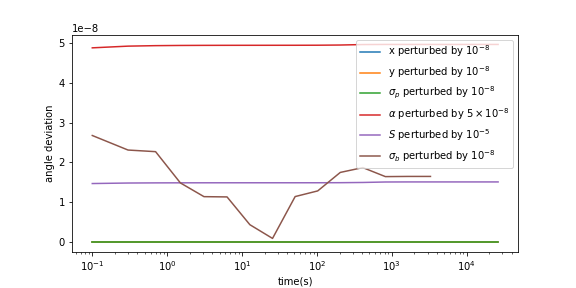
\includegraphics[width=12cm]{pertang.png}
		
		\caption{evolution of velocity amplitude and angle  after different perturbations}
		\label{pert}
	\end{figure}
	
		\begin{table}[!htb]
		\centering
		\label{pd}
		\caption{Partial derivatives and marginal errors}
		\begin{tabular}{llllllllllll}
			\toprule
			$\frac{\partial v}{\partial x}$ &$\frac{\partial v}{\partial y}$ &$\frac{\partial v}{\partial \sigma}$ &$\frac{\partial v}{\partial \alpha}$ &$\frac{\partial v}{\partial S}$ &$\frac{\partial v}{\partial \sigma_b}$& $\frac{\partial \theta}{\partial x}$ &$\frac{\partial \theta}{\partial y}$ &$\frac{\partial \theta}{\partial \sigma}$ &$\frac{\partial \theta}{\partial \alpha}$ &$\frac{\partial \theta}{\partial S}$ &$\frac{\partial \theta}{\partial \sigma_b}$	\\
			\midrule
			1.8e4 &	-2e7	& 1.6e11	& 3.3e15	&1.2e15	& 1.5e15 &0&0	&0 &4.96 &1.5	&1.8	\\
			\bottomrule
		\end{tabular}
		\begin{tabular}{llllll}
			\\
			\toprule
			$\Delta x$ & $\Delta y$ & $\Delta \sigma$ & $\Delta \alpha$ & $\Delta S$ & $\Delta \sigma_b$ \\
			\midrule
			2.54e-11m	&2.29e-15m	&2.16e-18m	&1.39e-21 rad	&3.81e-21$m^2$	&3.05e-21	\\
			\bottomrule
		\end{tabular}
	\end{table}
	
	In conclusion, the marginal error required by the system is unbelievably small. The location of the ground beam should be kept at atomic scale. The collimation of the beam should also be carefully calibrated to desired variance. The uniformity between different beams in the array should be strict so that the angle between different laser beam should be at scale of $10^{-21}$ rad. As for the fabrication, the error of the conic angle should be within $10^{-21}$ rad and error of area should be within $10^{-21}\,\,m^2$. However, if the payload is equipped with certain instrument that could actively adjust to the perturbation, the result might be better.
	
\bibliography{cit}
\bibliographystyle{plain}
\section{Appendix}
\subsection{Relativistic consideration}
\begin{figure}[htpb]
	\centering
	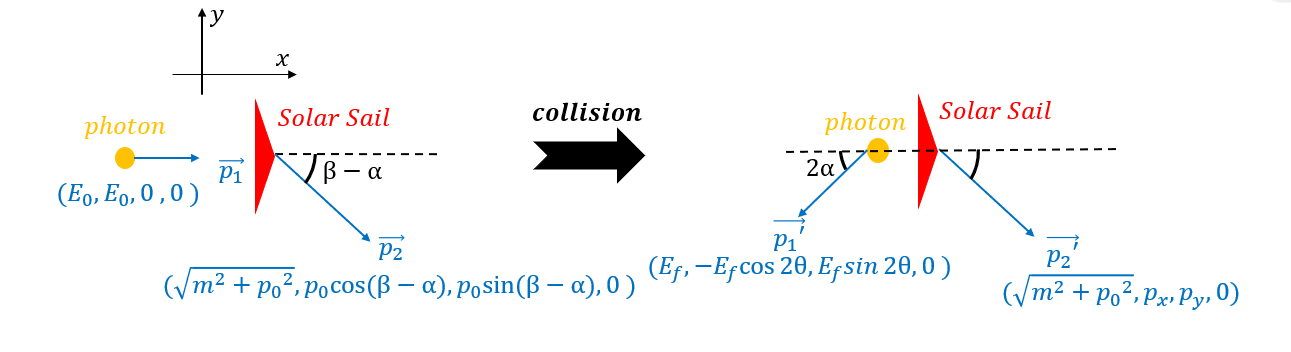
\includegraphics[width=12cm]{dyn.png}
	\caption{sketch of the photon pressure}
	\label{dyn}
\end{figure}
As shown in Fig. \ref{dyn}, we consider the collision between a photon and the light sail. With 4-momentum conservation (here natural unit is used, c=1):
\begin{equation}
	E_0+\sqrt{m^2+p_0^2} = E_f + \sqrt{m^2+p_x^2+p_y^2}
\end{equation}
\begin{equation}
	E_0+p_0\cos(\alpha-\theta) = -E_f \cos(2\theta) +p_x
\end{equation}
\begin{equation}
	p_0 \sin (\alpha-\theta) = E_f \sin(2\theta) + p_y
\end{equation}

With some algebraic derivation, we can solve $E_f,\, p_x,\, p_y$:

\begin{equation}
	E_f= \frac{E_0\sqrt{m^2+p_0^2} - E_0 p \cos (\alpha -\theta ) }{E_0-E_0 \cos(2\theta) + p_0 \cos (\alpha+\theta) +\sqrt{m^2+p_0^2} }
\end{equation}

\begin{equation}
p_x-p_0\cos(\alpha-\theta) = E_0+ E_f \cos(2\theta)
\label{f1}
\end{equation}

\begin{equation}
	p_y-p_0\sin (\alpha-\theta) = -E_f \sin(2\theta)
	\label{f2}
\end{equation}

Replace the $E_0$ with the laser power in (\ref{f1}) and (\ref{f2}) and recover the light speed in SI unit. We have the expression of force(here $\beta$ replaces $\theta$):
\begin{equation}
F_{//}=\int_S \frac{P(x) +P_f \cos (2\beta) }{c} dS 
\end{equation}
\begin{equation}
F_{\perp}=\int_S \frac{P_f \sin (2\beta)}{c} dS \\
\end{equation}
$F_{//}$ is the component parallel to the momentum and $F_\perp$ is the component perpendicular to the momentum.
$P_f$ is given by:
\begin{equation}
P_f=\frac{P(x) \sqrt{m^2c^4+|\vec{k}|^2c^2 } - P(x)|\vec{k}|c \cos(\alpha- \beta) }{P(x)dt (1-\cos(1\beta)) +\sqrt{m^2c^4+|\vec{k}|^2c^2 } + |\vec{k}|c \cos(\alpha- \beta) }
\end{equation}


\end{document}